\chapter{\textsf{\acronym}}
\section*{Descrição}
O NUXIS é uma ferramenta de gestão centralizada de recursos disponíveis numa rede. Consiste numa distribuição linux pré-instalada e configurada, que permite fazer a gestão via rede de servidores e seus recursos.

A \acronym encontra-se dividida principalmente em dois blocos funcionais:

\begin{itemize}
	\item \emph{Central Management} (CM)
        \item \emph{Virtualization Agent} (VA)
\end{itemize}

\begin{figure}[H]
	\begin{center}
	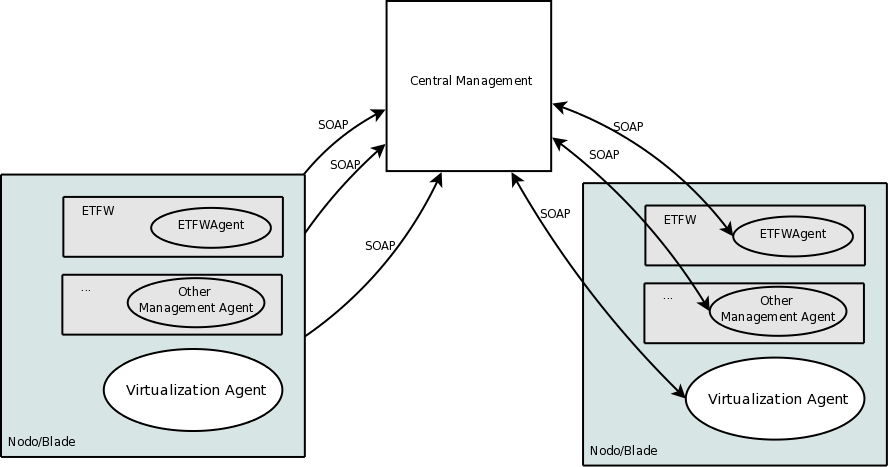
\includegraphics[scale=0.35]{screenshots/etva_blocos.png}
	\caption{Esquema geral do \acronym}
	\label{fig:etva_blocos}
	\end{center}
\end{figure}

O CM é o bloco responsável por gerir toda a infra-estrutura.
Os \emph{Virtualization Agents} são responsáveis pelo processamento dos pedidos entre os servidores de virtualização (\emph{nodes}) e o CM.

Dentro de um servidor de virtualização(\emph{node}) poderão existir máquinas virtuais com \emph{Management Agents}. Estes agentes, permitem a gestão ao nível dos serviços/aplicações instalados na máquina virtual (ver figura \ref{fig:etva_blocos} ).

No \acronym, existem vários servidores de virtualização (\emph{nodes}) a comunicar com o CM. A configuração da rede inicial, é efectuada, com recurso a VLANs, através do \emph{Assistente de configuração inicial} conforme indica a figura \ref{fig:first_time_wizard}.
\begin{figure}[H]
    \begin{center}
	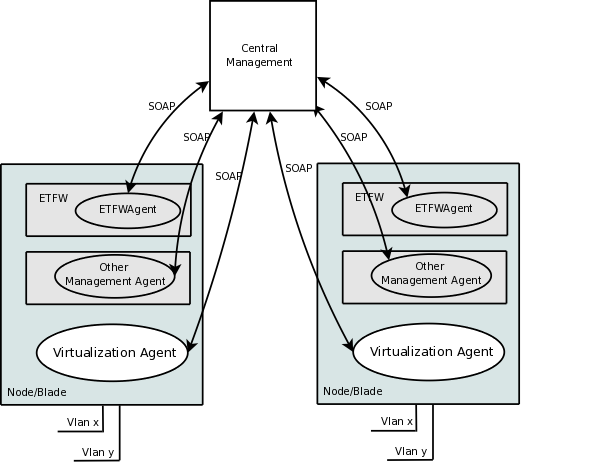
\includegraphics[scale=0.6]{screenshots/etva_enterprise.png}
	\caption{Modelo \acronym}
	\label{fig:etva_enterprise}
	\end{center}
\end{figure}
 
Este manual de utilização/configuração descreve a ferramenta de gestão, o CM (\emph{Central Management}).

\pagebreak
%\chapter{\textsf{Instalação}}
%\label{chp:installation}
%
%\pagebreak
